% !TEX root = ./nDICE.tex


\newboolean{useComma}
\setboolean{useComma}{true}


\section{Implementation and Empirical Evaluation}\label{sec:implementation}
In this section, we present a prototypical implementation of our inference engine and evaluate its efficiency.
The implementation is written in Ocaml and largely based on the existing \DICE library~\cite{holtzen2020scaling}, thus inheriting many of its features:
For instance, \NDICE inherits \DICE's relaxation of the A-normal form as well as its support for standard Boolean connectives and bounded numbers.
As the semantics of nondeterministic expressions depend on the order of evaluation, we define tuple elements and arguments of function calls to be evaluated from left to right.
By now, \DICE also supports bounded lists as well as an improved representation of numbers \cite{cao2023scaling}. 
We further provide a \texttt{choose}-statement to model the nondeterministic choice of a number from an interval.
Internally, all statements which choose or sample numbers are syntactic sugar for a sequence of flip operations and nested if-statements.
\DICE also switched the back-end for BDD operations from CUDD~\cite{somenzi2009cudd} to RSDD~\cite{RSDD}.
Since RSDD does not support ADDs, we implemented the ADD construction without a specialized library.
We further directly implemented Storm's bisection based algorithm \citeBisection, and use it to determine conditional reachability probabilities on MDPs to an accuracy of $10^{-6}$. 
We also use two optimizations\ext{}{, whose soundness is shown in the extended version \citeExtended}:
 
 
 \paragraph{Reduction to Boolean Programs}
 Consider some \NDICE expression $e$ of type $\BOOL \times \BOOL$, where we would like to infer the maximum probability to return $(\TRUE, \TRUE)$.
 Here, the standard construction creates an ADD with five output nodes: One for each value and one for the special value $R$.
 However, this construction creates unnecessary states in the MDP, as even though we care about the probability to reach $(\TRUE, \TRUE)$, additional states are included to distinguish whether the result will be $(\TRUE, \FALSE)$ or $(\FALSE, \TRUE)$.
 We can remove these states by instead determining the maximum probability that the expression $\LET{x = e}{x \leftrightarrow (\TRUE, \TRUE)}$ returns $\TRUE$.
 \ext{The soundness of this transformation is proven in \Cref{app:boolean_reduction}.}{}

 \paragraph{Probabilistic State Compression}
\begin{wrapfigure}[8]{r}{0.45\textwidth}
	\vspace*{-1\intextsep}%
	\begin{center}
		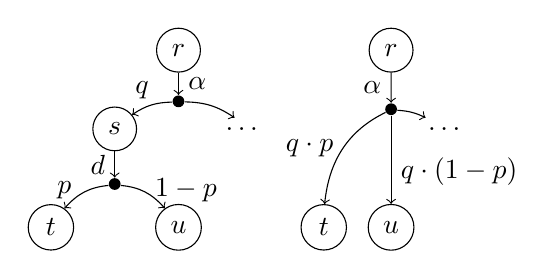
\begin{tikzpicture}[yscale=1, xscale=0.9]
			\node (i) at (0,0)   [draw, circle] {$r$};
			\node (s) at (-0.9,-1)   [draw, circle] {$s$};
			\node (dots) at (1,-1)   {$\dots\;\;$};
			\node (t) at (-1.8,-2.25)   [draw, circle] {$t$};
			\node (u) at (-0,-2.25)   [draw, circle] {$u$};
			
			\node (ro) at (0, -0.65)  [circle,fill,inner sep=1.5pt] {};
			\path[->]          (i)  edge   [bend right=0]   node[right, pos=0.5] {$\alpha$} (ro);
			\path[->]          (ro)  edge   [bend right=15]   node[above, pos=0.75] {$q$} (s);
			\path[->]          (ro)  edge   [bend right=-15]   node[above, pos=0.5] {} (dots);

			\node (so) at (-0.9, -1.7)  [circle,fill,inner sep=1.5pt] {};
			\path[->]          (s)  edge   [bend right=0]   node[left, pos=0.5] {$d$} (so);
			\path[->]          (so)  edge   [bend right=20]   node[left, pos=0.4] {$p\;$} (t);
			\path[->]          (so)  edge   [bend right=-20]   node[right, pos=0.4] {$\,1 - p$} (u);
			
%			\path[->]          (i)  edge   [bend right=20]   node[left] {$\alpha, q$} (s);
%			\path[->]          (i)  edge   [bend right=-20]   node[right] {} (dots);
			
%			\path[->]          (s)  edge   [bend right=20]   node[left] {$d, p$} (t);
%			\path[->]          (s)  edge   [bend right=-20]   node[right] {$d, 1-p$} (u);
			
			
			\def\offset{3};
			
			\node (i) at (0 + \offset,0)   [draw, circle] {$r$};
			\node (dots) at (0.75 + \offset,-1)   {$\dots$};
			\node (t) at (-0.95 + \offset,-2.25)   [draw, circle] {$t$};
			\node (u) at (0.0 + \offset,-2.25)   [draw, circle] {$u$};
			
			\node (io) at (0 + \offset, -0.75)  [circle,fill,inner sep=1.5pt] {};
			\path[->]          (i)  edge   [bend right=0]   node[left, pos=0.5] {$\alpha$} (io);
			\path[->]          (io)  edge   [bend right=30]   node[left, pos=0.5] {$q \cdot p$} (t);
			\path[->]          (io)  edge   [bend right=0]   node[right, pos=0.65] {$q \cdot (1-p)$} (u);
			\path[->]          (io)  edge   [bend right=-10]   node[above, pos=0.5] {} (dots);
			
%			\path[->]          (i)  edge   [bend right=20]   node[near end, left] {$\alpha, q \cdot p$} (t);
%			\path[->]          (i)  edge   [bend right=-0]   node[near end, right] {$\alpha, q \cdot (1-p)$} (u);
%			\path[->]          (i)  edge   [bend right=-20]   node[right] {} (dots);
		\end{tikzpicture}
	\end{center}
%	\caption{An example of state compression.}
%	\label{fig:compression}
\end{wrapfigure}
Intuitively, this removes states with a single enabled action by forwarding all incoming edges:
In the example on the right, state $s$ has a single enabled action $d$. 
Whenever we transit from $r$ via $\alpha$ to $s$ with probability $q$, we must subsequently transit via $d$ to either $t$ or $u$ with probabilities $p$  and $1-p$. 
Thus, we can remove $s$ from the MDP entirely and let $r$ transition via $\alpha$ directly to $t$ or $u$ with probabilities $q \cdot p$ and $q \cdot (1-q)$.
State compression can drastically reduce the size of MDPs in our use-case, as every state which represents a probabilistic flip can be removed.
\ext{We describe state compression formally in \Cref{app:compression}.}{}



\subsection{Empirical Performance Evaluation}\label{sec:ndet_empirical}
We will now perform an in-depth empirical evaluation aimed at investigating the overall efficiency and scalability of our inference method. 
To do so, we will consider a wide range of benchmarks of various sizes and with varying degrees of nondeterminism.
Regarding the evaluation itself, we will focus on answering the following questions:
\begin{itemize}
	\item[\textbf{Q1}:] \textbf{Scaling Behavior of the Compilation.}
	How quickly can the ADDs for \NDICE be compiled, and how does the needed time compare to the original compilation process of \DICE?
	\item[\textbf{Q2}:] \textbf{Reduction in the MDP State Space.}
	How much smaller are the MDPs constructed by \NDICE compared to a direct encoding of the same problem as an MDP? 
	\item[\textbf{Q3}:] \textbf{Inference Efficiency.} 
	How efficient is \NDICE inference compared to directly applying a probabilistic model checker?
	\item[\textbf{Q4}:] \textbf{Influence of Nondeterminism.}
	How does the amount of nondeterminism in a probabilistic program affect the runtime of \NDICE?
\end{itemize}
\noindent
For \textbf{Q1}, we will compare \NDICE with \DICE on purely probabilistic benchmarks.
To answer \textbf{Q2} and \textbf{Q3}, we encode each probabilistic program directly as an MDP, and we use Storm~\cite{hensel2022probabilistic} to infer the probabilities of the possible program outputs.
Storm offers multiple \enquote{engines} to internally represent MDPs, as well as different algorithms to perform model checking for conditional reachability probabilities.
The efficiency of model checking can heavily depend on the used configuration, and we made a best-effort attempt to identify and use the best combination.
As for benchmarks, PPLs typically do not consider nondeterminism -- existing benchmarks hence do not feature nondeterminism.
Thus, we introduce the following benchmark classes:


\begin{table}
	\caption{Performance of \NDICE on the benchmarks.
		The \DICE, \NDICE and Storm columns report the total runtime of the respective algorithm, \NDICE is run with state compression and split into \textit{compilation} and \textit{model checking}.
		$\NDICE_u$ reports the total inference time without state compression.
		All times are in ms, with a timeout (TO) after 20 minutes.
		\DICE runtimes are only reported for purely probabilistic benchmarks.
		The size of the MDP used by Storm is reported as $\text{MDP}_S$, whereas ADD Size and $\text{MDP}_n$ Size report the total size of the constructed ADDs and compressed MDPs for \NDICE.}
		
	\label{tab:Ndet}
	\begin{adjustbox}{max width=\textwidth}
	\begin{tabu}{c | c | ccc | c | c | c c c}
		\toprule
		Benchmark & \DICE & $\textit{comp.}$ & $\textit{checking}$ & \NDICE & $\NDICE_u$ & Storm & $\text{MDP}_S$ Size & ADD Size & $\text{MDP}_n$ Size \\
		\midrule
		Runway-7 & - & $8$ & $\approx 0$ & {$8$} & {$8$} & $18$ & $1.2 \times 10^3$ & $284$ & $40$ \\
		Runway-15 & - & $93$ & {$1 $} & {$94 $} & {$94 $} & {$131$} & $4.3 \times 10^4$ & $1.4\times 10^3 $ & $274$ \\
		Runway-30 & - & $531$ & {$7 $} & {$538 $} & {$538$ } & {$1\,620$} & $3.2 \times 10^5$ & $1.3\times 10^4 $ & $1.0\times 10^3$ \\
		Runway-40 & - & $999$ & {$11 $} & {$1\,010$} & {$1\,011 $} & {$5\,212$} & $7.5 \times 10^5$ & $2.4\times 10^4 $ & $1.8\times 10^3$ \\
		Runway-45 & - & $1\,514$ & {$15$} & {$1\,529$} & {$1\,530 $} & {$8\,673$} & $1.0 \times 10^6$ & $3.0 \times 10^4 $ & $2.2\times 10^3$ \\
				
		\midrule
		CouponProb-10 & 
				$721$ &
		$1\,379$ & {$\approx 0$} & {$1\,379$} & 
		{$1\,379$} & $5\,894$ &
		 $1.2 \times 10^6$ & $3.4\times10^5$ & $8$ \\
		CouponProb-11 & 
				$1\,958$ & 
		$3\,904$ & {$\approx 0$} & {$3\,904$} & 
		{$3\,904$} & $18\,839$ &
		 $3.4 \times 10^6$ & $8.3\times10^5$ & $8$ \\
		CouponProb-12 & 
				$5\,798$ & 
		$10\,484$ & {$\approx 0$} & {$10\,484$} & 
		{$10\,484$} & $56\,434$ &
		 $8.7 \times 10^6$ & $2.0\times10^6$ & $8$ \\
		CouponProb-13 & 
				$20\,691$ & 
		$32\,153$ & {$\approx 0$} & {$32\,153$} & 
		{$32\,153$} & $171\,358$ &
		 $2.2 \times 10^7$ & $4.8\times10^6$ & $8$ \\
		CouponProb-14 & 
				$63\,418$ & 
		$96\,068$ & {$\approx 0$} & {$96\,068$} & 
		{$96\,068$} & $641\,614$ &
		 $5.5 \times 10^7$ & $1.1\times10^7$ & $8$ \\
		
		\midrule
		CouponNdet-6 & - & $105$ &  {$14$} & {$119$} & {$120$} & $162$ & $6.9 \times 10^4$ & $1.9\times10^4 $ & $818$ \\
		CouponNdet-7 & - & $276$ & {$41$} & {$317$} & {$317$} & $607$ & $2.1 \times 10^5$ & $5.6\times10^4 $ & $1.9\times10^3$ \\
		CouponNdet-8 & - & $731$ & {$96$} & {$827$} & {$824$} & $2\,208$ & $6.3 \times 10^5$ & $1.5\times10^5 $ & $5.2\times10^3$ \\
		CouponNdet-9 & - & $2\,264$ & {$389$} & {$2\,653$} & {$2\,662$} & $8\,110$ & $1.7 \times 10^6$ & $4.3\times10^5 $ & $1.4\times10^4$ \\
		CouponNdet-10 & - & $6\,105$ & {$1\,257$} & {$7\,362$} & {$7\,293$} & $25\,862$ & $4.8 \times 10^6$ & $1.0\times10^6 $ & $3.9\times10^4$ \\
		
		\midrule
		Network-2000 & - & $2\,218$ & {$24$} & {$2\,242$} & {$2\,242$} & $25$ & $1.2 \times 10^4$ & $2.4\times10^4$ & $8.0\times10^3$ \\
		Network-4000 & - & $9\,530$ & {$55$} & {$9\,585$} & {$9\,585$} & $39$ & $2.4 \times 10^4$ & $4.8\times10^4$ & $1.6\times10^4$ \\
		Network-6000 & - & $22\,270$ & {$84$} & {$22\,354$} & {$22\,358$} & $54$ & $3.6 \times 10^4$ & $7.2\times10^4$ & $2.4\times10^4$ \\
		Network-8000 & - & $40\,763$ & {$122$} & {$40\,885$} & {$40\,885$} & $68$ & $4.8 \times 10^4$ & $9.6\times10^4$ & $3.2\times10^4$ \\
		Network-10000 & - & $67\,081$ & {$153$} & {$67\,234$} & {$67\,243$} & $84$ & $6.0 \times 10^4$ & $1.2\times10^5$ & $4.0\times10^4$ \\
		
		\midrule
		Rabin-50 & - & $324$ & {$\approx 0$} & {$ 324$} & {$ 324 $} & $17$ & $5.2 \times 10^3 $ & $524 $ & $206 $ \\
		Rabin-100 & - & $1\,962 $ & {$1$} & {$ 1\,963 $} & {$ 1\,963 $} & $23$ & $2.0 \times 10^4$  & $1.0 \times 10^3 $ & $406 $ \\
		{Rabin-250} & - & $23\,355 $ & {$2$} & {$ 23\,357 $} & {$ 23\,357 $} & $82$ & $1.2 \times 10^5$ & $2.8 \times 10^3 $ & $1.0 \times 10^3$ \\
		{Rabin-500} & - & $233\,494 $ & {$6$} & {$233\,500$} & {$233\,501$} & $327$ & $5.0 \times 10^5$ & $5.8 \times 10^3 $ & $2.0 \times 10^3 $ \\
		
		\midrule 
		Survey & $1$ & $1$ & $\approx 0$ & $1$ & $1$ & $14$ & $238$ & $71$ & $14$ \\
		Hepar2 & $99$ & $309$ & $\approx 0$ & $309$ & $310$ & $23\,094$ & $1.8 \times 10^{19} $ & $1.8 \times 10^4$ & $8$ \\
		Insurance & $580$ & $2\,227$ & $\approx 0$ & $2\,227$ & $2\,232$ & $9\,460$ & $4.2 \times 10^{11}$ & $1.5 \times 10^5$ & $16$ \\
		Water & $9\,241$ & $9\,288$ & $\approx 0$ & $9\,288$  & $9\,347$   & $12\,545$ & $2.4 \times 10^{9} $ & $5.2 \times 10^4$ & $16$ \\
		Alarm & $160\,104$ & $161\,385$ & $\approx 0$ & $161\,385$ & $161\,385$ & $5\,335$ & $1.8 \times 10^{16}$ & $1.2 \times 10^5$ & $14$ \\
		
		\midrule 
		Survey-Ndet & - & $1$ & $\approx 0$ & $1$ & $1$ & $14$ & $238$ & $71$ & $26$ \\
		Hepar2-Ndet & - & $280$ & $14$ & $294$ & $295$ & $23\,909$ & $1.8 \times 10^{19} $  & $1.8 \times 10^4$ & $2.0 \times 10^3$ \\
		Insurance-Ndet & - & $2\,217$ & $\approx 0$ & $2\,217$ & $2\,220$ & $10\,345$ & $4.2 \times 10^{11}$ & $1.5 \times 10^5$ & $56$ \\
		Water-Ndet & - & $9\,296$ & $\approx 0$ & $9\,296$ & $9\,298$ & $13\,153$ & $2.4 \times 10^{9} $ & $5.2 \times 10^4$ & $56$ \\
		Alarm-Ndet & - & $161\,786$ & $47$ & $161\,633$ & $161\,636$ & $5\,219$ & $1.8 \times 10^{16}$ & $1.2 \times 10^5$ & $6.9 \times 10^3$ \\
		
		
		\midrule
		3sat-0 & $19\,511$ & $19\,535$  & {$\approx 0$} & {$19\,535$} & {$19\,535$} & TO & $1.2 \times10^{13}$ & $4.7\times10^4$ & $8$ \\
		3sat-25 & - & $19\,528$ & {$43$} & {$19\,571$} & {$19\,571$} & TO & $1.2 \times10^{13}$ & $4.7\times10^4$ & $1.2\times10^4$ \\
		3sat-50 & - & $19\,544$ & {$69$} & {$19\,613$} & {$19\,612$} & TO & {$1.2 \times10^{13}$} & $4.7\times10^4$ & $2.3\times10^4$ \\
		3sat-75 & - & $19\,514$ & {$72$} & {$19\,586$} & {$19\,584$} & TO & {$1.2 \times10^{13}$} & $4.7\times10^4$ & $3.6\times10^4$ \\
		3sat-100 & - & $19\,567$ & {$107$} & {$19\,674$} & {$19\,676$} & TO & {$1.2 \times10^{13}$} & $4.7\times10^4$ & $4.7\times10^4$ \\
		\bottomrule
	\end{tabu}
	\end{adjustbox}
\end{table}

\paragraph{Runway}
We consider the adapted vehicle tracking problem from \citet{junges2021runtime} as presented in \Cref{sec:overview}, but with more locations for the ground vehicle, more measurements, and a vehicle which may move up to two locations per time step.
In particular, the benchmark \textit{runway-n} refers to the scenario with $n$ possible locations for the ground vehicle and $n$ measurements of the vehicle position.
In this class of benchmarks, roughly $10\%$ of all flip operations are nondeterministic.

\paragraph{Coupon Collector}
We consider a variation of the Coupon Collector Problem inspired by \citet{jansen2016bounded}:
A collector aims to collect $N$ distinct coupons within $N$ rounds.
In every round, the collector may draw \emph{two} coupons from a bowl.
An observe statement enforces that the two coupons are distinct.
We consider two instances of this problem: One where the coupons are always drawn from a uniform distribution (\textit{CouponProb}), and one where we nondeterministically choose between three bowls with different distributions each round (\textit{CouponNdet}).
\textit{CouponProb} is purely probabilistic, whereas for \textit{CouponNdet} roughly $14\%$ of flip operations are nondeterministic. 

\paragraph{Network Reachability} 
We consider a network reachability problem adapted by \citet{holtzen2020scaling} from \citet{gehr2018bayonet}, and then further extended with nondeterminism by us.
Here, server~$S_1$ forwards an incoming packet to either $S_2$ or $S_3$, which in turn forward the packets to $S_4$, but $S_3$ drops packets with probability $0.1\%$.
For load balancing, $S_1$ chooses randomly between $S_2$ or $S_3$, and nondeterministically between three protocols.
This benchmark is scaled up by repeating this forwarding process, and roughly $25\%$ of all flips are nondeterministic.

\paragraph{Fair Exchange}
We consider a case study of the Prism Model Checker \cite{KNP11}, namely the probabilistic fair exchange protocol from \citet{rabin1983transaction}.
The protocol allows two parties to exchange commitments to a pre-defined contract with the aid of a trusted third party.
Nondeterminism is used to model a bad actor, and we infer the maximum probability that one party commits to the contract while the bad actor doesn't.
Here, over $95\%$ of flip operations are nondeterministic.

\paragraph{Bayesian Networks}
Similar to \DICE~\cite{holtzen2020scaling}, we evaluate \NDICE on some well-known Bayesian networks from the the Bayesian Network Repository\footnote{\url{https://www.bnlearn.com/bnrepository/}}, namely \textit{Survey}, \textit{Hepar2}, \textit{Insurance}, \textit{Water} and \textit{Alarm}.
We consider two instances for each network: A purely probabilistic version which directly encodes the Bayesian network as a \NDICE program, and a version were some parent-less nodes behave nondeterministically.
Here, nondeterminism can model behaviors which may be influenced by non-probabilistic factors.
For example, a  patient may lie about their alcoholism, and a network which models their diagnosis can reflect this uncertainty with nondeterminism.
The amount of nondeterminism varies heavily between networks, ranging from $5\%$ of flips being nondeterministic for \textit{Insurance-Ndet} to up to $30\%$ of flips being nondeterministic for \textit{Alarm-Ndet}.

\paragraph{3SAT} 
We consider a 3SAT problem based on a benchmark retrieved from \citet{hoos2000satlib}
with $40$ variables and $114$ clauses encoded as a \NDICE program.
This benchmark is not scaled by increasing the program size, but instead we increase the amount of nondeterministic variables. 
For example, \textit{3sat-25} is an instance where $25\%$ of the $40$ variables are assigned a value nondeterministically and the remaining variables randomly.
\medskip


The performance of \DICE, \NDICE and Storm on these benchmarks is presented in \Cref{tab:Ndet}.
The considered inference task was to determine the maximum probability for all outputs of the input program.
\NDICE is run with state compression and split into $\mathit{comp.}$ for the construction of the MDPs and \textit{checking} to determine conditional reachability probabilities.
We report the total runtime without state compression as $\NDICE_u$.
We also list the number of states in the MDP used by Storm as \enquote{$\text{MDP}_S$ Size}, as well as the total size of the ADDs and the total number of MDP states \emph{after} state compression as used by \NDICE.
All experiments were run on macOS Sonoma 14.5 with a 3.49 GHz Apple M2 Pro chip and 32~GB RAM.
Benchmarks were run 5 times and \Cref{tab:Ndet} reports the average runtime; standard deviations are reported in \ext{\Cref{app:extended_results}}{the extended version \citeExtended}.

For Storm, we used the following engines: The benchmarks classes \textit{Runway}, \textit{CouponProb} and \textit{CouponNdet} required conditional reachability properties, which are only supported by the \enquote{sparse} engine.	
Here, the \textit{Coupon} benchmarks performed best with the \enquote{restart} algorithm by \citet{baier2014computing}, whereas the \textit{Runway} benchmarks used Storm's custom \enquote{bisection} algorithm to determine conditional probabilities. 
Beyond that, the \textit{Network} and \textit{Rabin} benchmarks as well as the \textit{Survey} Bayesian network performed best with the \enquote{sparse} engine, whereas the remaining benchmarks preferred the symbolic \enquote{dd} engine.
We now turn our attention to the previously posed questions:



%How quickly can the ADDs for \NDICE be compiled, and how does the needed time compare to the original compilation process of \DICE?
\subsubsection*{Q1: Scaling Behavior of the Compilation.}
To answer this question, we will primarily consider the performance of \DICE and \NDICE on the probabilistic Coupon Collector and Bayesian network problems. 
We observe that the compilation time of \NDICE is slower than \DICE, likely because \NDICE does not use a dedicated decision diagram library to construct ADDs.
Still, the compilation time of noDice scales similarly to Dice on the Coupon Collector benchmarks, where \NDICE takes about twice as long as the more specialized \DICE, and their compilation times are comparable on most Bayesian networks.
Since the model checking times on these benchmarks are negligible for noDice, we can conclude that  \NDICE is slower than \DICE on purely probabilistic programs, but both approaches scale similarly for larger programs.


%How much smaller are the MDPs constructed by \NDICE compared to a simpler encoding of the same problem?
\subsubsection*{Q2: Reduction in the MDP State Space.}
Overall, \NDICE is consistently able to construct significantly smaller MDPs than the direct encoding for the same benchmark problems.
More precisely, the \DICE-style compilation is able to avoid an exponential blow-up of the ADDs by exploiting local structure in the programs, leading to the ADDs themselves usually already being much smaller than the MDPs build by Storm.
The \textit{Network} benchmarks form an exception to this, since \NDICE requires more MDP states than Storm to infer all values.
After all, these benchmarks contain no redundancy which is not already exploited by Storm.
Thus, both \NDICE and Storm build MDPs of the same size, but Storm constructs one MDP which is used to infer the probabilities for both output values, whereas \NDICE builds separate MDPs for the two values, leading to a total state space which is twice as large.
Beyond that, state compression is able to reduce the state space of the MDPs even further depending on the amount of nondeterminism in the benchmark.
In particular, state compression yields larger reductions on problems with less nondeterminism.


%How efficient is \NDICE inference compared to other approaches?
\subsubsection*{Q3: Inference Efficiency.}
	Looking at \NDICE, we observe that compilation takes the vast majority of the runtime, whereas model checking takes little to no time in comparison.
	This behavior is consistent with \DICE, which also spends most of the runtime on the compilation, but performs the weighted model count, meaning \DICE's equivalent to model checking, within milliseconds.
	For both \NDICE and \DICE, quick model checking is the result of the large reduction in the state space due to the use of decision diagrams in the compilation process.
	However, the further reduction of the MDP size with state compression did not speed up \NDICE inference in a meaningful way, since the runtimes of \NDICE and $\NDICE_u$ are almost identical.
	
	We will now compare the performance of \NDICE and Storm.
	 We first note that \NDICE outperforms Storm on several problems, namely the \textit{Runway}, \textit{Coupon Collector} and \textit{3sat} benchmarks along with most Bayesian networks.
	On these problems, the small MDPs of \NDICE allow for highly efficient model checking, whereas Storm constructs much larger MDPs which are expensive to construct and model check.
	Still, \NDICE's compilation is not always worth it, as seen with the \textit{Network} and \textit{Rabin} benchmarks:
	Here, the compilation of a small MDP by \NDICE is far too costly compared to Storm, which solves these problems in milliseconds.
	
	This raises the question as to when \NDICE is faster than simply using Storm.
	Judging from the results in \Cref{tab:Ndet}, we believe that a key distinguishing characteristic between the performance of Storm and \NDICE is the dimensionality of the state space.
	Put differently, Storm performs better on problems where only a few variables are needed to describe the state space, whereas \NDICE favors benchmarks which include many variables.
	As an example, the \textit{Network} benchmark can be encoded with just 2 variables: The current status of the package and the remaining number of rounds. 
	In contrast, the \textit{Coupon} benchmarks require many variables more, as every coupon requires a variable to track whether it has already been obtained.
	Storm struggles with the resulting high dimensionality, since it enumerates the reachable states, while \NDICE combines states which behave similarly.
	We do however note that the \textit{Alarm} Bayesian network forms an exception to this intuition, since \NDICE performs surprisingly bad whereas Storm performs surprisingly well.


%How does the amount of nondeterminism in a probabilistic program affect the runtime of \NDICE?
\subsubsection*{Q4: Influence of Nondeterminism.}
Overall, the share of nondeterministic flip operations does not significantly influence the runtime of \NDICE.
This is best demonstrated with the \textit{3SAT} benchmarks:
Here, both the compilation time as well as the ADD size are unaffected by the number of nondeterministic variables, whereas the compressed MDP size and the time spent on model checking increase.
The same effect can also be observed when comparing the probabilistic and nondeterministic instances of the Bayesian network benchmarks, as compilation times are largely unaffected and model checking is a little slower.
This is to be expected, as the ADD construction is agnostic to the nature of flip operations, whereas model checking treats the flips differently depending on their nature.
However, the overall time spent on model checking remains negligible compared to the compilation, and thus the amount of nondeterminism in a benchmark does not significantly affect the overall runtime.


\medskip



In summary, \NDICE is able to construct compact MDPs for rather large programs, speeding up the inference procedure as a whole.
Thanks to this, the inference process is able to outperform state-of-the-art model checkers on a variety of benchmarks, but the construction of the MDP can be very expensive for other benchmarks classes.
Due to this, we believe that \NDICE is particularly suited for problems which contain a large number of variables, leading to a high dimensionality of the state space.
Beyond that, state compression can further reduce the size of the MDP for \NDICE, but this reduction does not translate to faster inference.
Overall, we believe that our prototype implementation serves as a proof of concept that a \NDICE-style algorithm can efficiently perform inference for probabilistic programs with nondeterminism. 



